\documentclass[12pt]{article}


\usepackage[fleqn]{amsmath}
\usepackage{amssymb}
\usepackage{graphicx}

\usepackage{caption}
% \usepackage{subcaption}

\usepackage{subfig}
% \usepackage{subcaption}
% \graphicspath{ {C:/Users/Indy-Windows/Documents/EEC-289A-RL/HW/HW1/latex_file/images/}}
\graphicspath{ {images/}}


\usepackage{hyperref}
\hypersetup{
colorlinks=false,
linkcolor=blue,
filecolor=magenta,
    urlcolor=blue,
}
\urlstyle{same}



\begin{document}


\title{ EEC-289A Reinforcement Learning \\ Homework \#1 }


\author{Jonathan~Dorsey \\\url{https://github.com/JonnyD1117/EEC-289A-RL/tree/main/HW}}
\maketitle




\section*{ $\varepsilon$-Greedy}

\subsection*{Algorithm Implementation} The $ \varepsilon$ -Greedy algorithm was implemented as close as possible to the given algorithm in the course text.

\begin{enumerate}
    \item Initialize any parameters and constants
    \item Iterate over the total number of trials (2000)
    \item Sample actual rewards for k = 10 problem from Normal distributions
    \item Initialize action values (Q) and number of action selections (N) to arays of zero
    \item Within this outter loop iterate over the total number of time steps (1000)
    \item Sample $varepsilon$ from a uniform distribution from 0 to 1
    \item With probability $p = 1 - \varepsilon$  select the maximal action (greedy)
    \item With probability $p = \varepsilon$ select a random action
    \item Compute reward for given action
    \item Update action values (Q) and number of actions selections (N)
    \item Collect reward data over all iterations and plot

\end{enumerate}


\section*{Upper-Confidence-Bound}

The only material difference between the \textbf{UCB} algorithm and the \textbf{$\varepsilon $ -Greedy} algorithm, is the action section. Instead of select the action according to a value of $ \varepsilon$ evaluated at each iteration of the loop by drawing a sample from a uniform distribution, the \textbf{UCB} algorithm leverages the action value update law by considering the amount of times an action has been selected as well as the current timestep. As we sample from the actions, the more often that certains actions are selected via UCB, the lower \underline{effective-variance} the action value will be. This can be seen by the fact that as the number of action selections (for a particular action) goes to infinity, the quantity in the squareroot will trend to zero, which would effectively state that the variance in the value associated with that action is zero.


$$
A_{t} \doteq \underset{a}{\arg \max }\left[Q_{t}(a)+c \sqrt{\frac{\ln t}{N_{t}(a)}}\right]
$$

By implementing this as the means of action selection (instead of stoichastic sample used in $\varepsilon$ - Greedy), we can obtain the UCB algorithm.

\subsection*{Reproducability}

To the best of my knowledge, I had no issues with reproducing the results shown in the textbook, within numerical precision. As mentioned in the text, there is a noticeable spike in reward at the 11th time step, which is faithfully reproduced in the plots I generated vai my own implementation.


\subsection*{Figures}

Both the Figure 2.4 from the Sutton \& Barto text and the equivalent generated plots from my personal matlab code are shown below.

\subsubsection*{Program Run Times}

\begin{itemize}
    \item $\varepsilon$-Greedy: 24 seconds
    \item Upper-Confidence-Bound: 30 seconds
\end{itemize}


\begin{figure}[ht]%
    \centering
    \subfloat[\centering Fig: 2.4 from Sutten \& Barto ]{{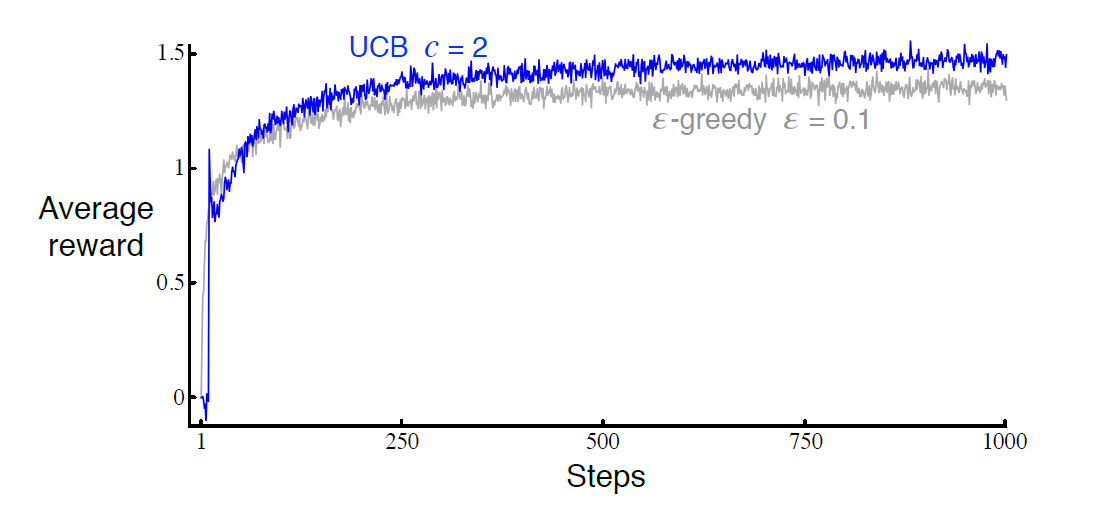
\includegraphics[width=.9\linewidth]{book_egreedy} }}%
    \\
    \subfloat[\centering Generated Results from Matlab Code]{{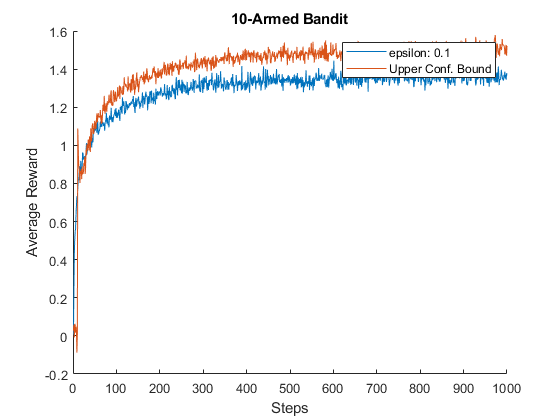
\includegraphics[width=.75\linewidth]{upper_conf_bound} }}%
    % \caption{Pose-to-Pose MPC Curves:}%
    % \label{fig:pose2pose_control_action}%
\end{figure}













\end{document}
